\section{Auswertung}
\label{sec:Auswertung}


\subsubsection{(a) Erzeugen einer amplitudenmodulierten Schwingung mit
Hilfe eines Ringmodulators}
\label{subsubsec:auswertung_a}

\begin{figure}
  \centering
  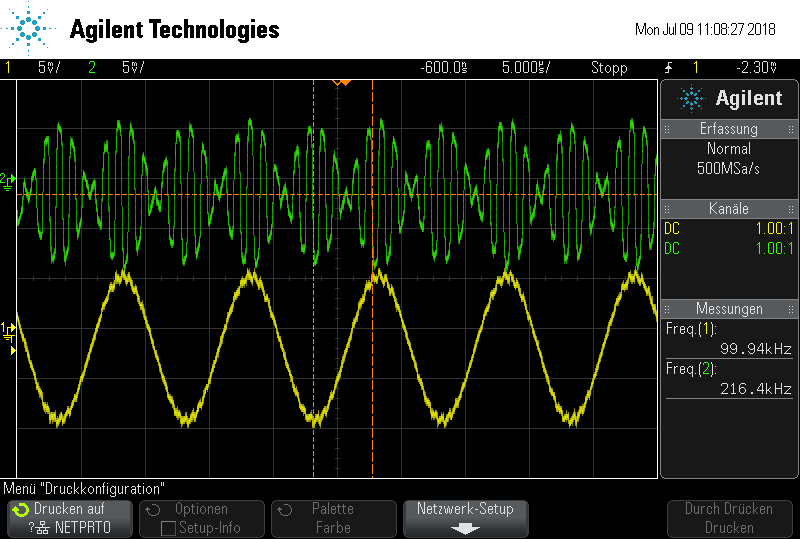
\includegraphics[width=0.7\textwidth]{osci/amp_ringmodulator.png}
  \caption{Amplitudenmodulierte
  Schwingung eines Ringmodulators.}
  \label{fig:ringamp_zeit}
\end{figure}


\subsubsection{(b) Untersuchung des Frequenzspektrums einer
amplitudenmodulierten Schwingung}
\label{subsubsec:auswertung_b}

\begin{figure}
  \centering
  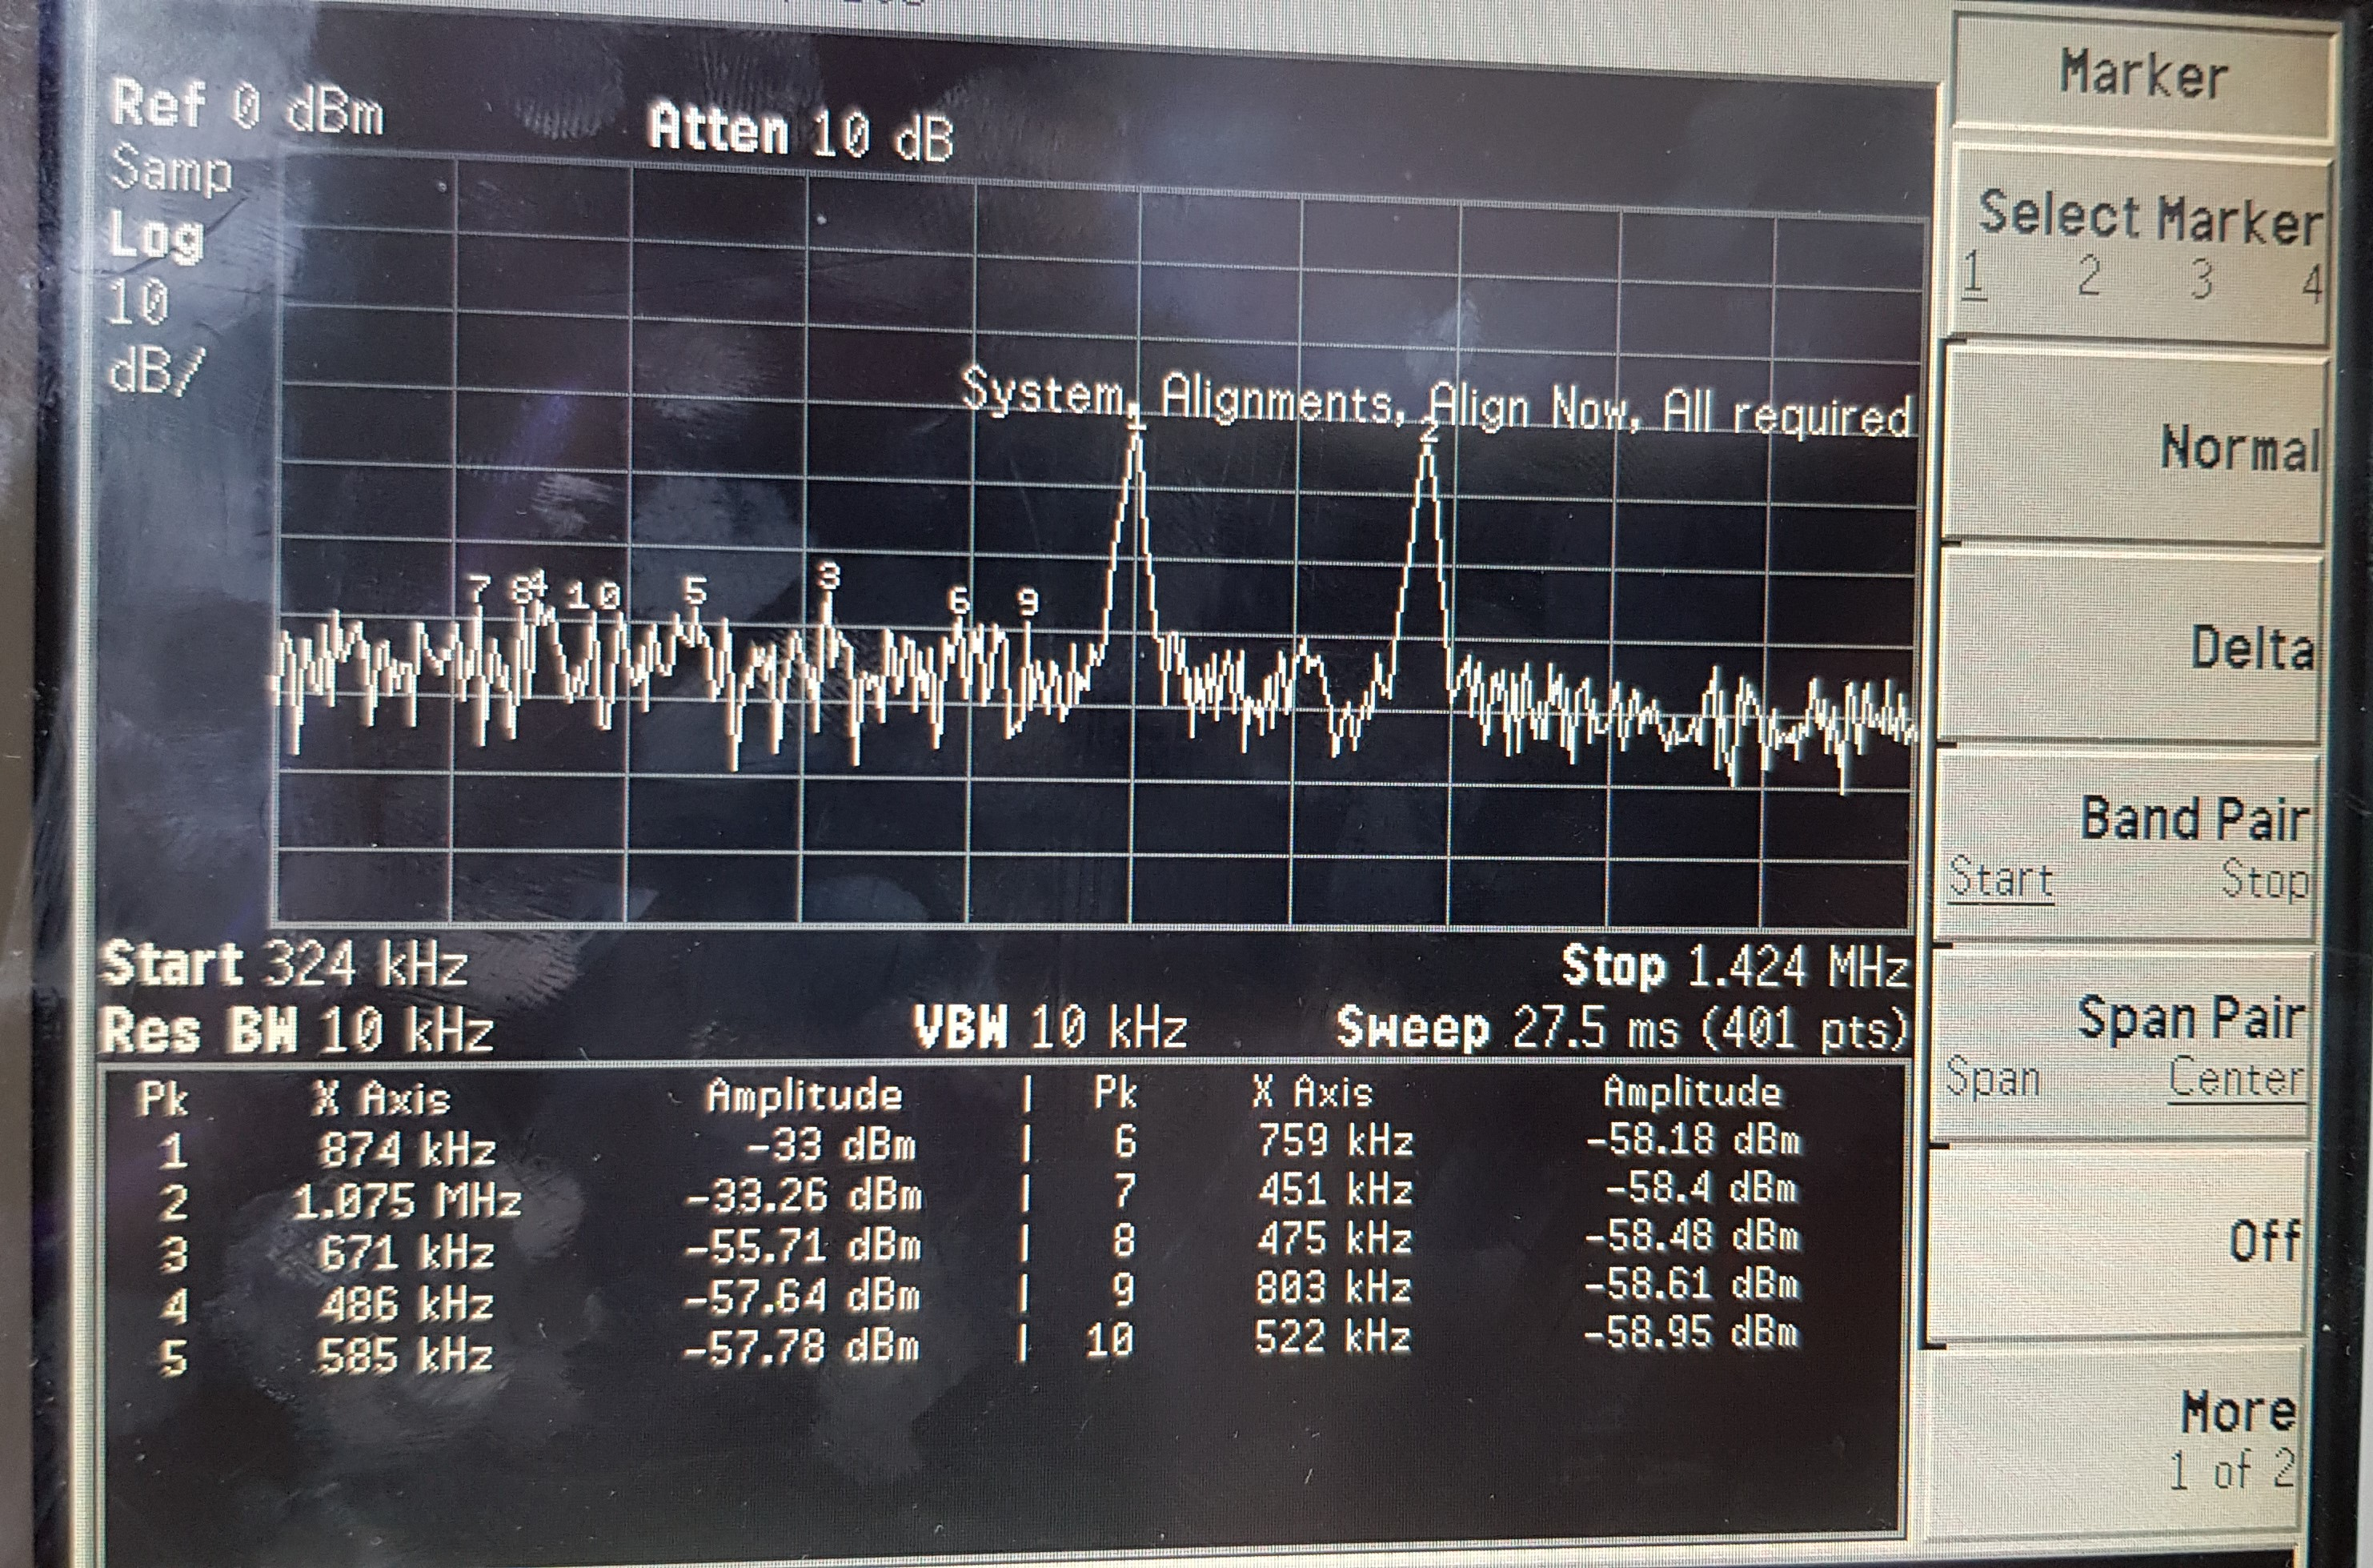
\includegraphics[width=0.7\textwidth]{spec/frequenzbereich_klein_ring.png}
  \caption{Amplitudenmodulierte
  Schwingung eines Ringmodulators im Frequenzraum.}
  \label{fig:ringamp_frequenz}
\end{figure}



\subsubsection{(c) Erzeugen einer amplitudenmodulierten Schwingung
mit Hilfe einer Gleichrichterdiode}
\label{subsubsec:auswertung_c}

\begin{figure}
  \centering
  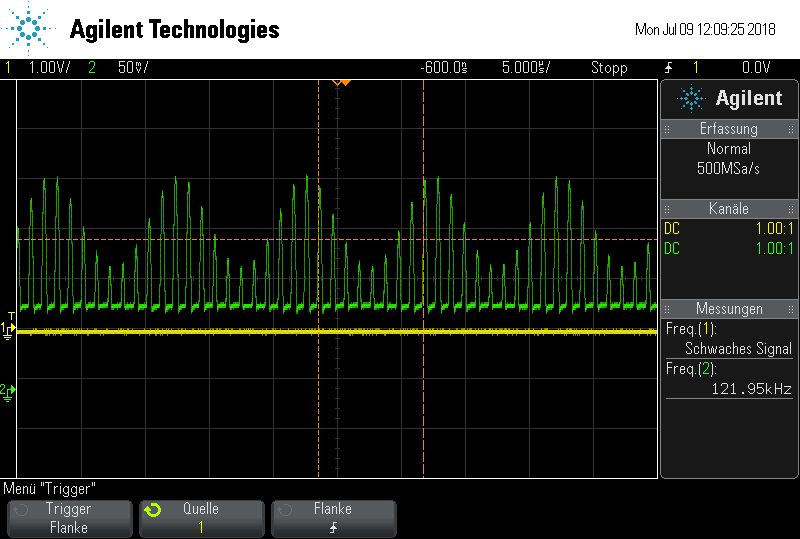
\includegraphics[width=0.7\textwidth]{osci/amp_diode.png}
  \caption{Amplitudenmodulierte
  Schwingung einer Diode nach dem Aufbau aus Abb.\ref{fig:13}.}
  \label{fig:diode_zeit}
\end{figure}


\begin{figure}
  \centering
  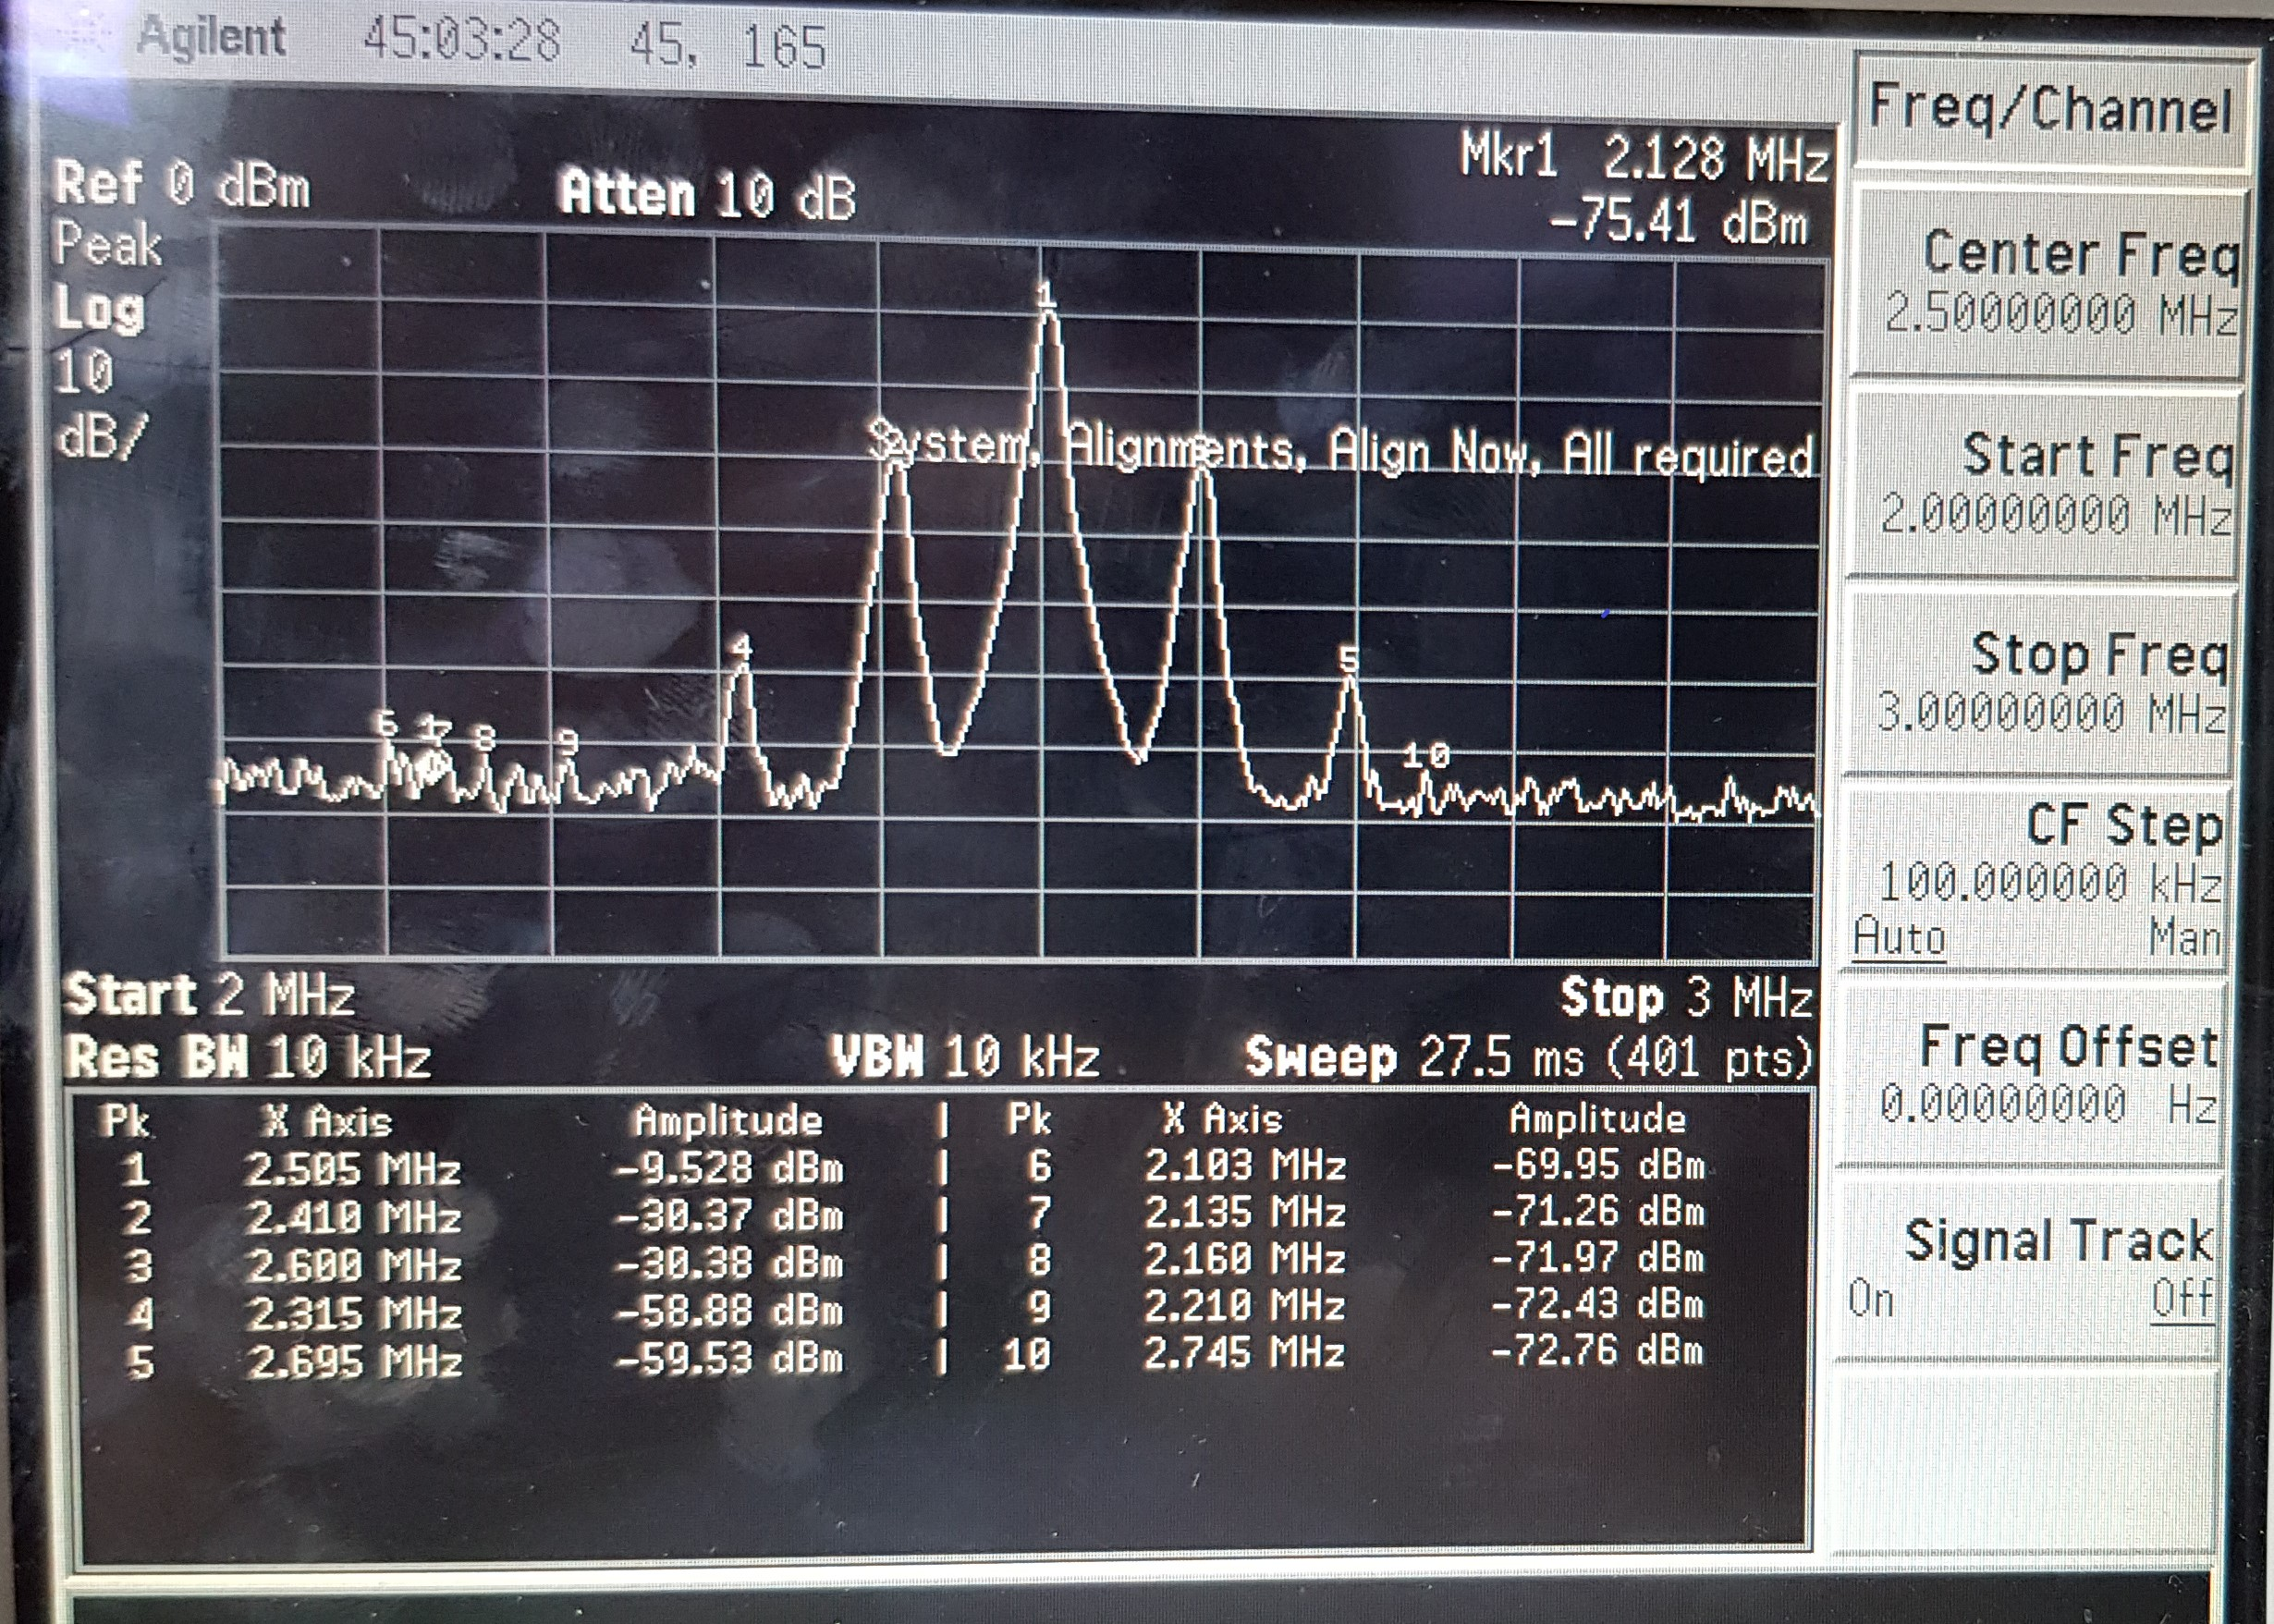
\includegraphics[width=0.7\textwidth]{spec/frequenzbereich_klein_diode.jpg}
  \caption{Amplitudenmodulierte
Schwingung einer Diode im Frequenzraum.}
  \label{fig:diode_frequenz_klein}
\end{figure}


\begin{figure}
  \centering
  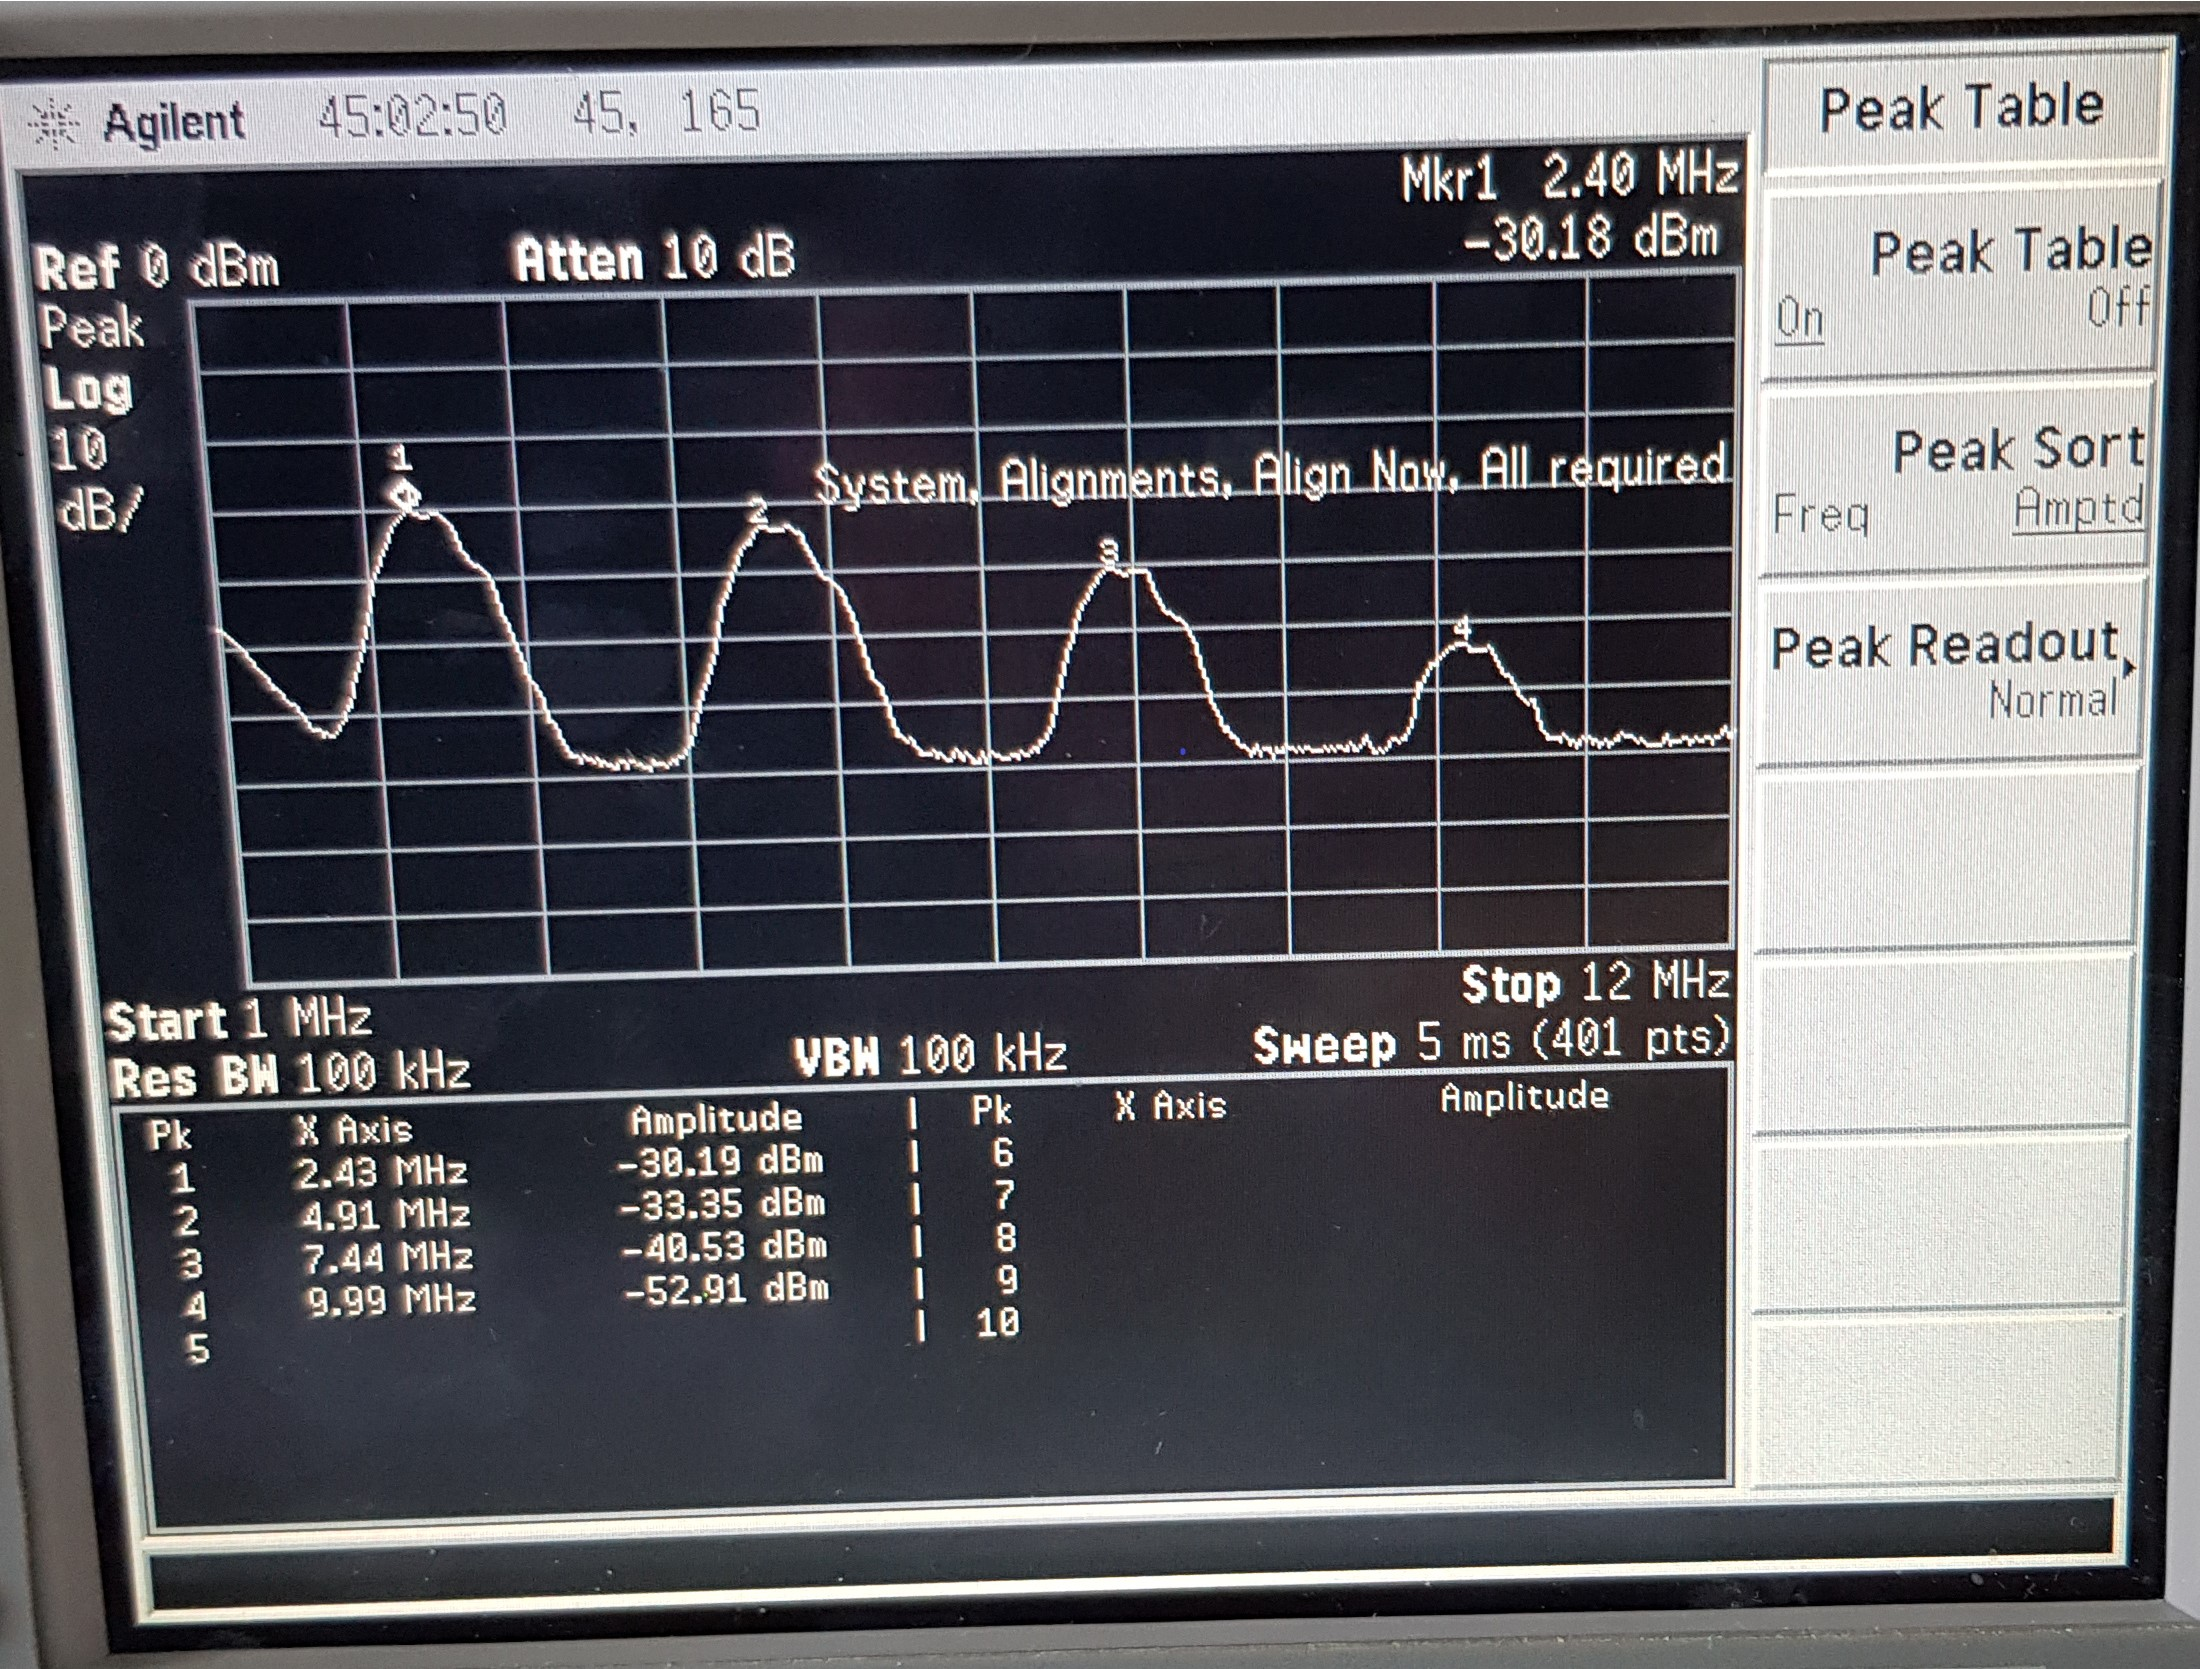
\includegraphics[width=0.7\textwidth]{spec/frequenzbereich_gross_diode.jpg}
  \caption{Amplitudenmodulierte
Schwingung einer Diode im Frequenzraum mit Oberschwingungen.}
\label{fig:diode_frequenz_gross}
\end{figure}




\subsubsection{(d) Erzeugen einer frequenzmodulierten Schwingung}
\label{subsubsec:auswertung_d}

\begin{figure}
  \centering
  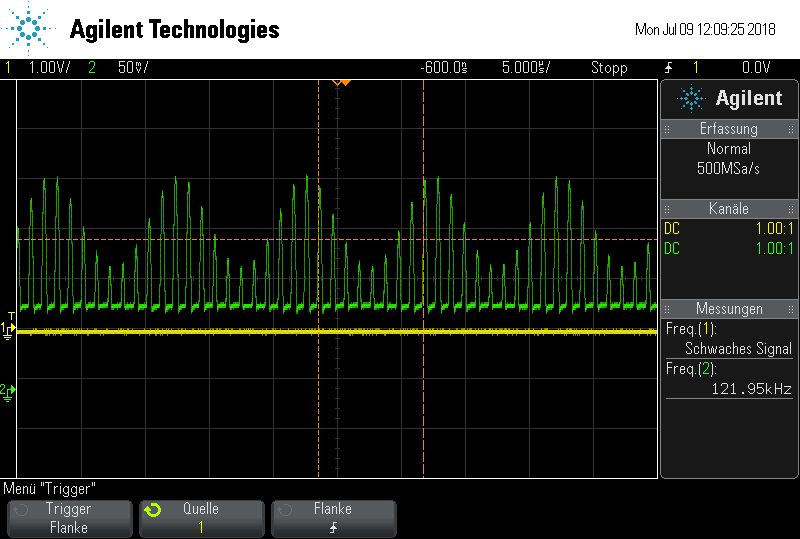
\includegraphics[width=0.7\textwidth]{osci/amp_diode.png}
  \caption{Frequenzmodulierte
  Schwingung erzeugt nach dem Aufbau aus Abb.\ref{fig:15}.}
  \label{fig:frequ_zeit}
\end{figure}


\begin{figure}
  \centering
  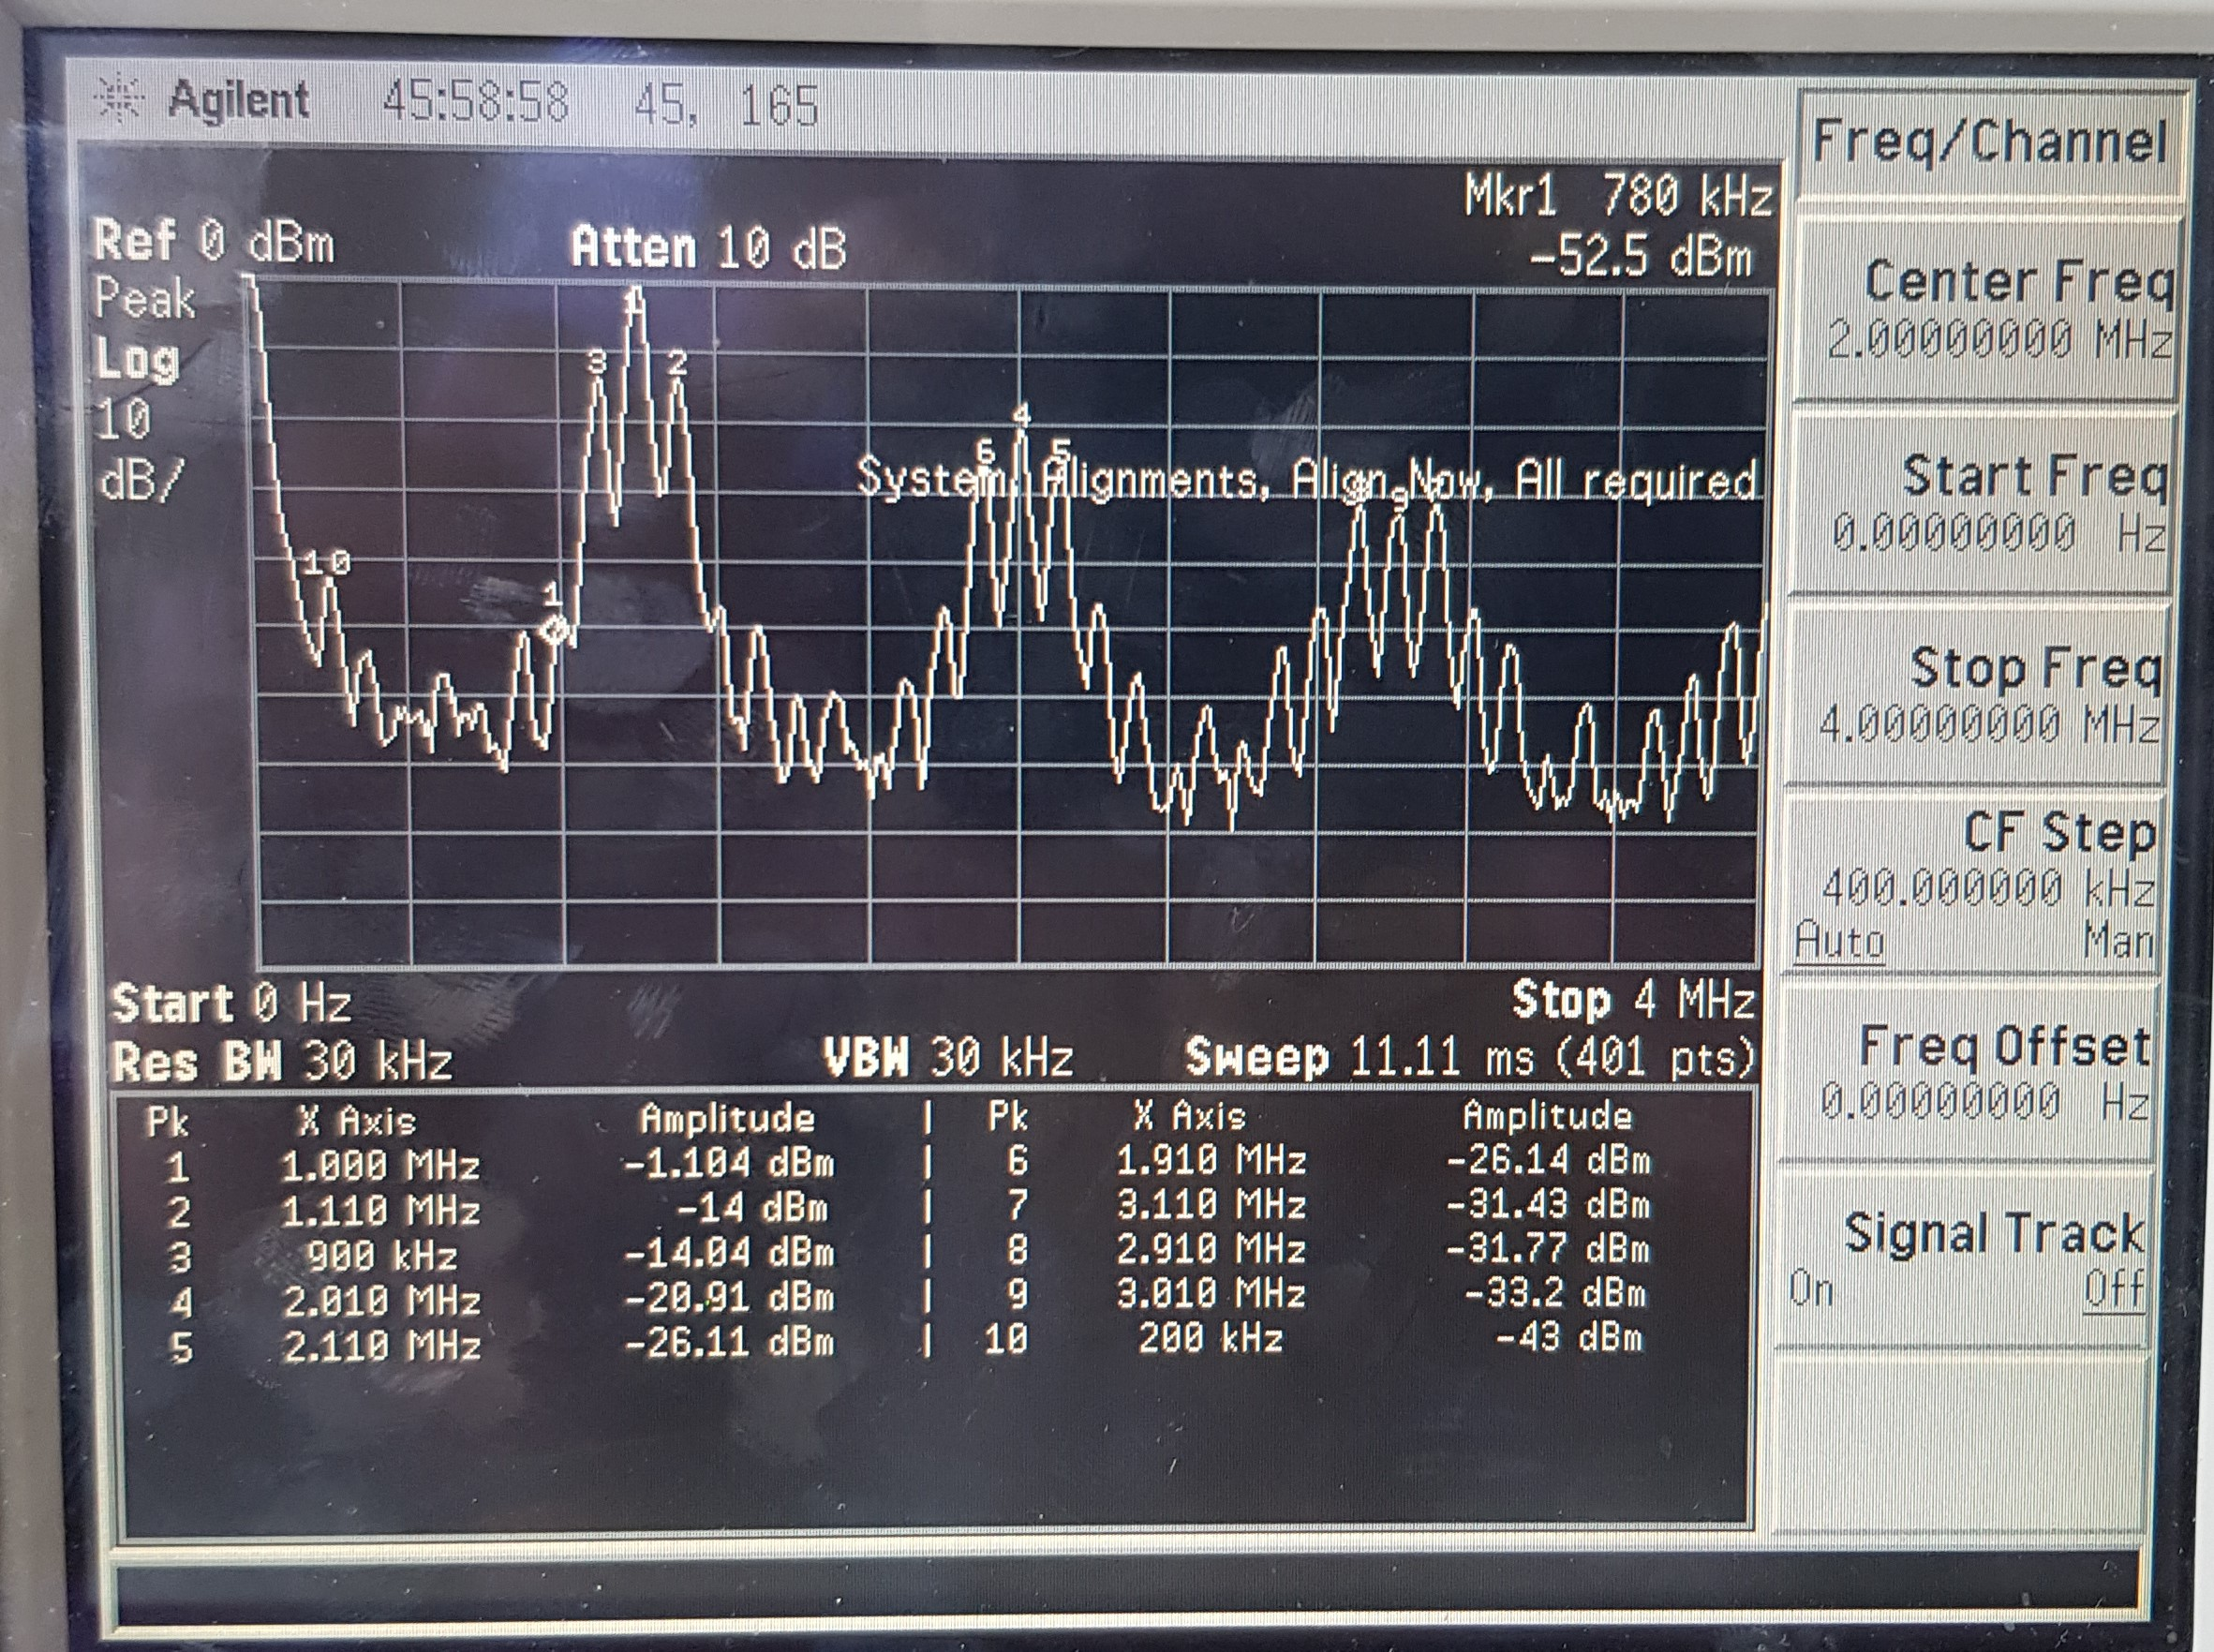
\includegraphics[width=0.7\textwidth]{spec/frequenzmodulation_bereich_fresh_cool.jpg}
  \caption{Frequenzmodulierte
Schwingung im Frequenzraum.}
\label{fig:diode_frequenz_gross}
\end{figure}




\subsubsection{(e) Untersuchung der Phasenabhängigkeit eines
phasenempfindlichen Gleichrichters}
\label{subsubsec:auswertung_e}

\begin{figure}
  \centering
  \includegraphics[width=0.7\textwidth]{build/plot.pdf}
  \caption{Amplitude in Abhängigkeit von der Phase.}
  \label{fig:plot}
\end{figure}

\subsubsection{(f) Demodulation einer amplitudenmodulierten Schwingung
mit Hilfe eines Ringmodulators}
\label{subsubsec:auswertung_f}

\begin{figure}
  \centering
  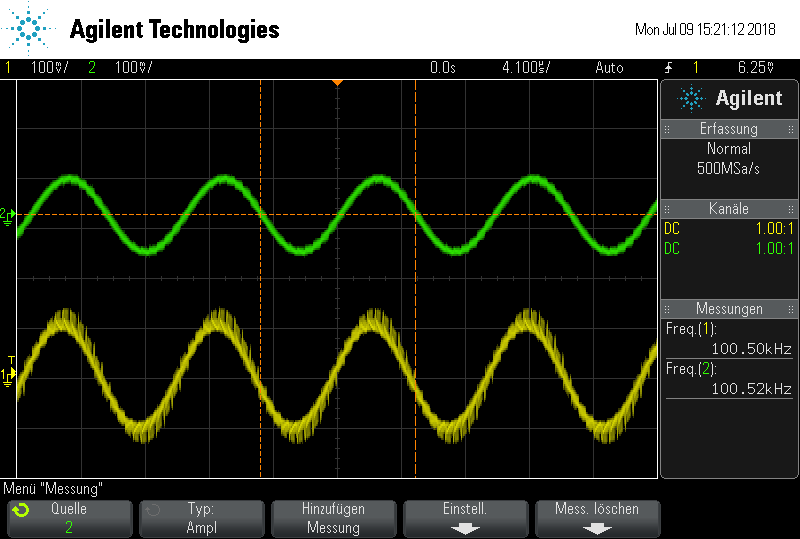
\includegraphics[width=0.7\textwidth]{osci/amp_demod.png}
  \caption{Demodulation von amplitudenmoduliertem Signal mit Hilfe eines
  Ringmodulator nach Schaltung \ref{fig:7}.}
  \label{fig:amp_demod_ring}
\end{figure}




\subsubsection{(g) Demodulation einer amplitudenmodulierten Schwingung
mit Hilfe einer Gleichrichterdiode}
\label{subsubsec:auswertung_g}

\begin{figure}
  \centering
  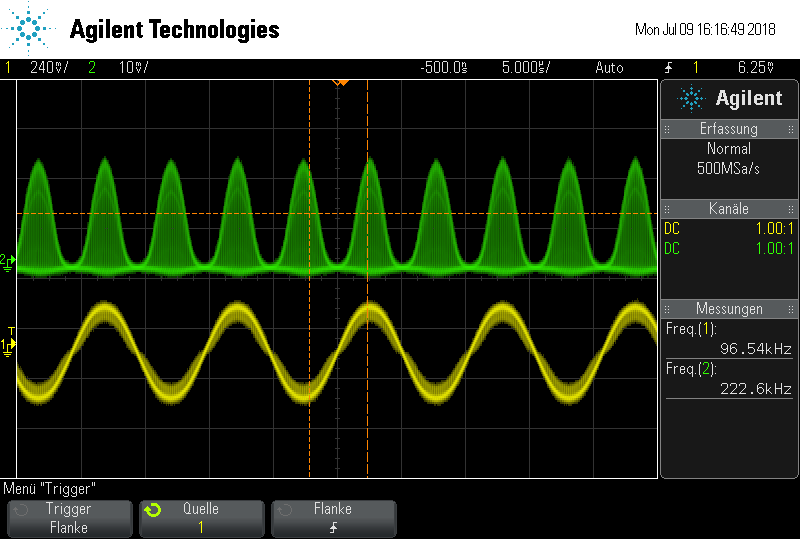
\includegraphics[width=0.7\textwidth]{osci/amp_demod_diode_A.png}
  \caption{Signal am Punkt A bei der Demodulation von amplitudenmoduliertem Signal mit Hilfe einer
  Diode und einem Tiefpass nach Schaltung \ref{fig:8}.}
  \label{fig:diode_punkt_A}
\end{figure}


\begin{figure}
  \centering
  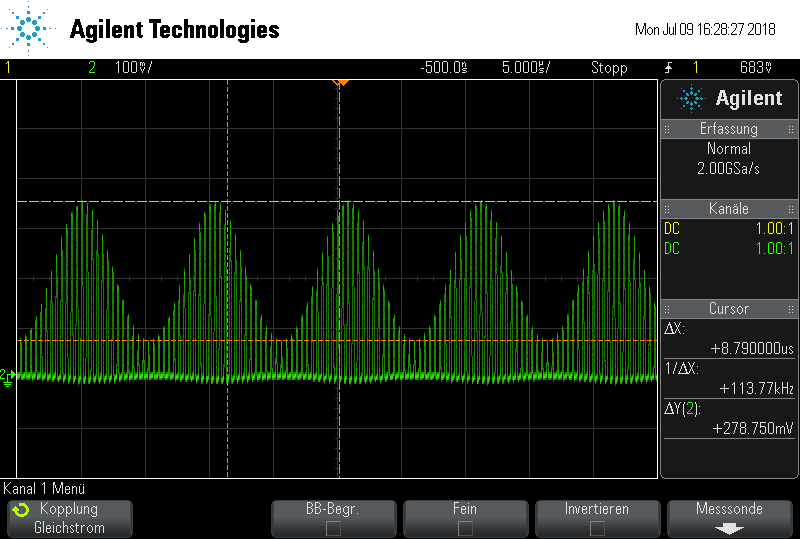
\includegraphics[width=0.7\textwidth]{osci/amp_demod_diode.png}
  \caption{Demoduliertes Signal von einem amplitudenmoduliertem Signal mit Hilfe einer
  Diode und einem Tiefpass nach Schaltung \ref{fig:8}.}
  \label{fig:diode_demod_amp}
\end{figure}



\subsubsection{(h) Demoduolation einer frequenzmodulierten Schwingung
mit Hilfe eines Flankendemodulators}
\label{subsubsec:auswertung_h}

\begin{figure}
  \centering
  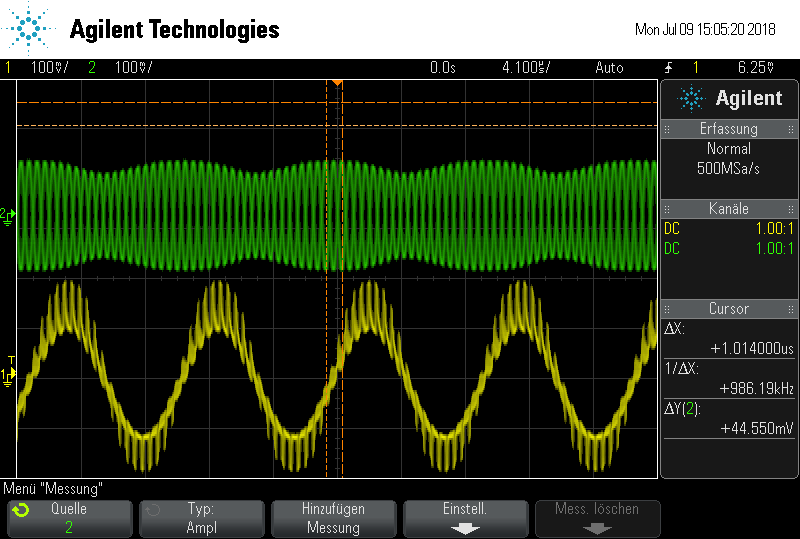
\includegraphics[width=0.7\textwidth]{osci/freq_demod_amp.png}
  \caption{Umwandelung eines Frequenzmodulierten Signales in ein Amplitudenmoduliertes
Signal mit durch einen Schwingkreis nach Abbildung \ref{fig:11}.}
\label{fig:freq_zu_amp}
\end{figure}



\begin{figure}
  \centering
  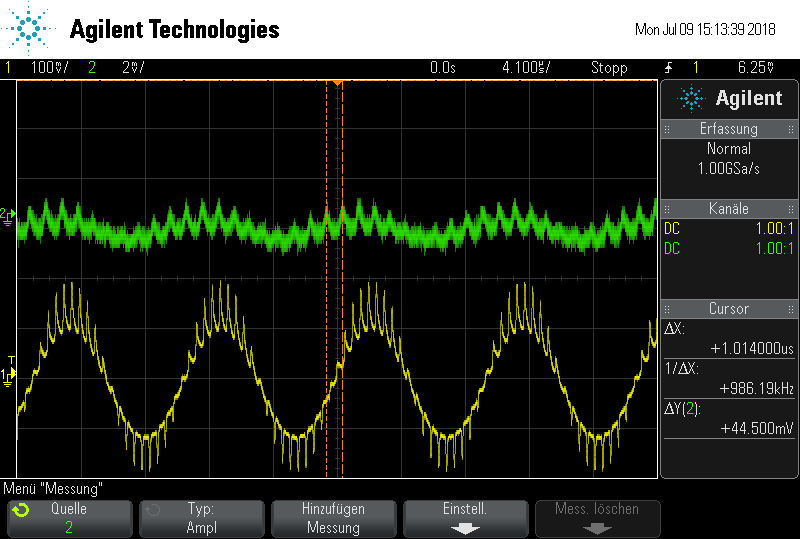
\includegraphics[width=0.7\textwidth]{osci/freq_demod.png}
  \caption{Demodulierung eines frequenzmodulierten Signales
  mit der Schaltung \ref{fig:11}.}
\label{fig:demod_frequenz}
\end{figure}
